In this section we describe the experiments that are performed and show some results. In the section of the qualitative results we give some visualizations of the topics that are found with the different models. We show that the topics can be meaningful and that semantic descriptions can be given to some of the topics.\\
In the section of the quantitative results we compare the two developed models with each other and show the performance for different number of topics and different number of time-slices.

% Wat wil ik nou eigenlijk aantonen en kan ik dat ook aantonen?
% Ik wil aantonen dat het nieuwe model werkt. Ik wil aantonen dat het beter werkt dan normal LDA model. 
% Het is al door meerdere mensen aangetoond dat topic modellen wel van nut zijn om behavior patronen in sensor data te vinden.
% en we kunnen dus aantonen dat onze nieuwe methode OOK werkt, want we kunnen patterns vinden. eg: een dag in de week is de persoon in de middag weg, of 's nachts moet die persoon naar het toilet

% QUALITATIVE EXPERIMENTEN
%Ik wil aantonen dat mijn model werkt en dat je wel zinnige informatie eruit kunt halen. Je kunt een semantische omschrijving van de topics geven.
%We vergelijken de nieuwe method met de BOW/k-means methode we kunnen hier ook aangeven wat de verhoudingen zijn van worden in de data en unique worden die zijn gevonden. Dit geeft ook al aan dat BOW waarschijnlijk niet werkt


%Met de gegeven data en de gekozen feature representation zijn we niet in staat om zinnige informatie uit de BOW model te halen.

% QUANTITATIVE EXPERIMENTEN


% In this section we first give some qualitative results, where the topic distribution on some days are shown. 
% Then we do something else
% Then we compare the BIC's?
% And after that we make a small test according to the feature representation.


%To test the performance of the topic models we set the variables of the features to fixed values.  In the basic LDA model we use a coarse grain value for the time. This means that the sixth dimension can have 5 different values, where the time intervals are $\{ 3am - 8am, 8am - 1pm, 1pm - 18pm, 18pm - 23pm, 23pm - 3am  \}$.
\subsection{Qualitative Results}
In the following some visualizations of the different models are shown. First the topic distributions over some days are represented, for the different models. There are four model compared with each other. The first two models are the LDA model with a Bag-of-word representation with and without pre-clustering the dictionary with k-means. The other two model are the LDA-Gaussian model and the LDA-Poisson model which are described above.\\
After that a more detailed view of the topics is given and some semantic meanings of the topics are described.\\

For the visualization of the topics every time-slice is marked with a different color. The color depends on the topic that the time-slice belongs to. The belonging topic is the one with the highest probability of the observation in the given time-slice.



\subsubsection{Comparison of the different models}
In the following figures we used $N=96$ time-slices for a day. The time dimension has a coarse-grain representation of the time, which means that there are five different time values. The number of topics that are initialized are $k=5$.
With the given representation the LDA model with a BOW-representation is still able to find different topics in the data, although the BOW representation without the clustering only distinguish between two topics (see figure \ref{fig:bow96}). If the data is clustered on forehand LDA is able to find four different topics in the data (see figure \ref{fig:kMeans96}). The number of clusters for the k-means algorithms is set to $V=6$.

\begin{figure}[h!]
 \centering
 \begin{minipage}[b]{0.45\linewidth}
  \centering
  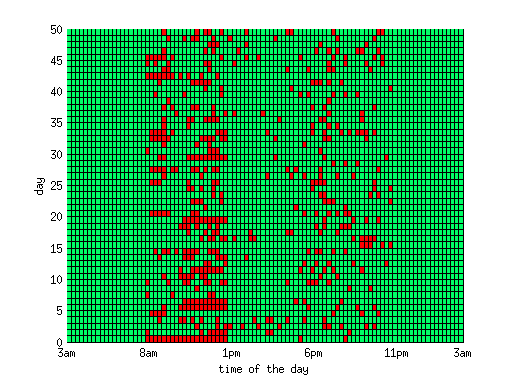
\includegraphics[width=\textwidth]{Pictures/DayTopicsTs96k5bow.png}
  \caption{Topic distribution for 50 days for the Bag-of-Words model}
  \label{fig:bow96}
 \end{minipage}
 \begin{minipage}[b]{0.45\linewidth}
  \centering
  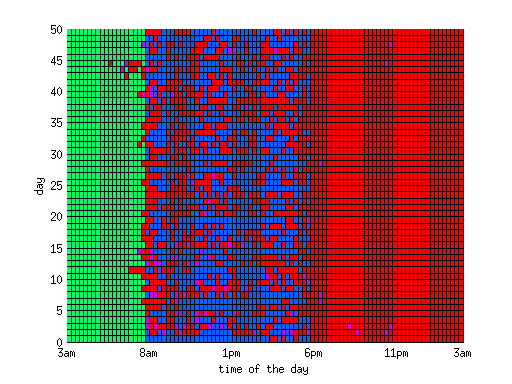
\includegraphics[width=\textwidth]{Pictures/DayTopicsTs96k5Clus.png}
  \caption{Topic distribution for 50 days for the k-means model}
  \label{fig:kMeans96}
 \end{minipage}
 \caption{}
\end{figure}



In figure \ref{fig:Pois96} the outcome of the LDA-Poisson model is shown with the same variable values as before. On the right-hand side of the figure the topic description of the five topics that are found. The colors of the topics in the two images are equal to each other, so every red time slice on the left image is the topic that is shown with red in the right image. The six dimension of the observations are shown in this figure (\ref{fig:PoisTopVisu96}) on the x-axis. On the y-axis of every subfigure the $\lambda$-value of the Poisson distribution is shown. You can see (figure \ref{fig:PoisDay96}) that the LDA-Poisson model gives a relative high priority on the time value, because every day is separated into three timezones (yellow,green,red) and only the two other topics (blue, purple) are generated with respect of the sensor values of the five fields.

\begin{figure}
 \centering
 \begin{minipage}[b]{0.45\linewidth}
  \centering
  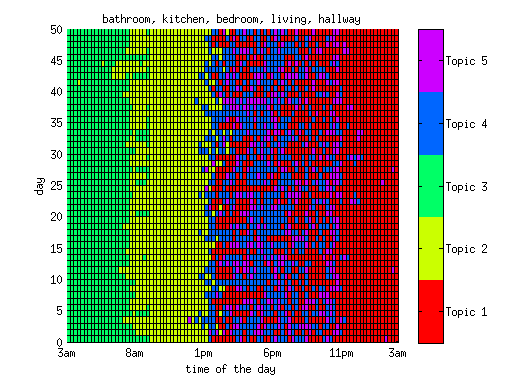
\includegraphics[width=\textwidth]{Pictures/TopDayHN3TS96k5Pois.png}
  \caption{Topic distribution for 50 days}
  \label{fig:PoisDay96}
 \end{minipage}
 \begin{minipage}[b]{0.45\linewidth}
  \centering
  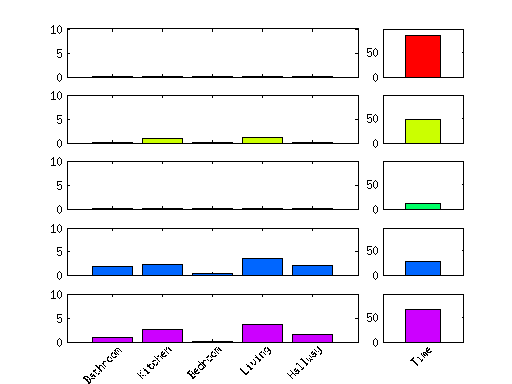
\includegraphics[width=\textwidth]{Pictures/TopVisuHN3TS96k5Pois.png}
  \caption{Visualization of the topics}
  \label{fig:PoisTopVisu96}
 \end{minipage}
 \caption{Topic distribution per day and the Topic visualization for LDA-Poisson}
 \label{fig:Pois96}
\end{figure}


Figure \ref{fig:Gaus96} shows the outcome of the LDA-Gaussian model again with the same variable values. In the right figure (\ref{fig:GausTopVisu96}) on the x-axis again the 6 dimensions of the observations are shown. On the y-axis the mean value $\mu$ of the Gaussian distribution is shown and in the bar-chart the standard deviation $\sigma$ is given with a vertical black line. You can see that the red topic here has a high $\sigma$-value and captures all time-slice where no sensor data is measured. The purple topic seems to represent the 'Going to the toilet at night' topic. Here the mean value of the time is low and only a few sensor measurements are captured. You can see that this model captures more sophisticated topics, that represent more meaningful results.

\begin{figure}
 \centering
 \begin{minipage}[b]{0.45\linewidth}
  \centering
  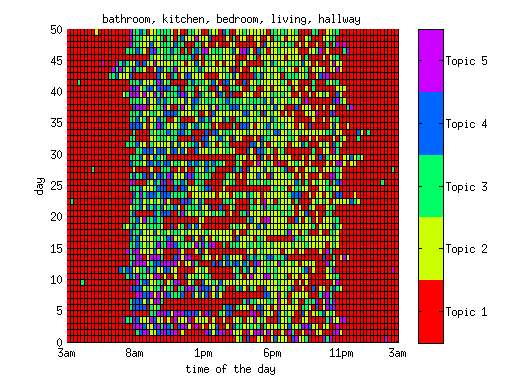
\includegraphics[width=\textwidth]{Pictures/TopDayTS96k5Gaus.png}
  \caption{Topic distribution for 10 days}
 \end{minipage}
 \begin{minipage}[b]{0.45\linewidth}
  \centering
  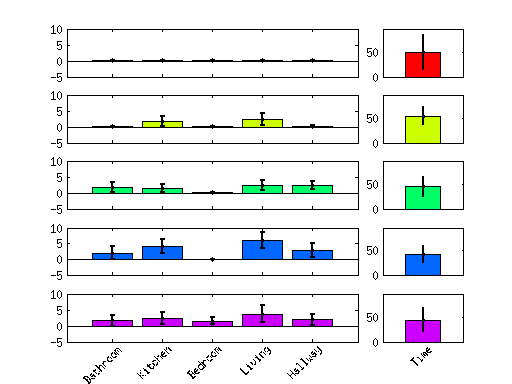
\includegraphics[width=\textwidth]{Pictures/TopVisuTS96k5Gaus.png}
  \caption{Visualization of the topics}
  \label{fig:GausTopVisu96}
 \end{minipage}
 \caption{Topic distribution per day and the Topic visualization for LDA-Gaussian}
 \label{fig:Gaus96}
\end{figure}

\subsubsection{An attempt for semantic topic description}
In the following figures the topic distribution for the five different houses is shown for the two models, LDA-Gaussian and LDA-Poisson. The number of time-slices is set set to $N=48$ and the models are initialized with $k=20$ topics and the time has a fine-grain representation. For every house and model 50 days of the data is shown. The ten topics with highest value are shown, time-slices that belong to a different topic are marked with gray.
%-----------------------------------------------------------
%% HN=1
\begin{figure}
 \centering
 \begin{minipage}[b]{0.45\linewidth}
  \centering
  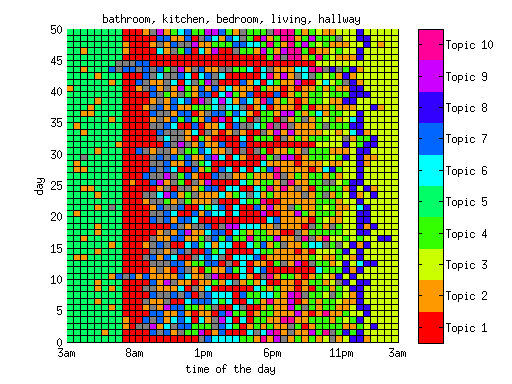
\includegraphics[width=\textwidth]{Pictures/Gaus/DayHN1TS48k20.png}
 \end{minipage}
 \begin{minipage}[b]{0.45\linewidth}
  \centering
  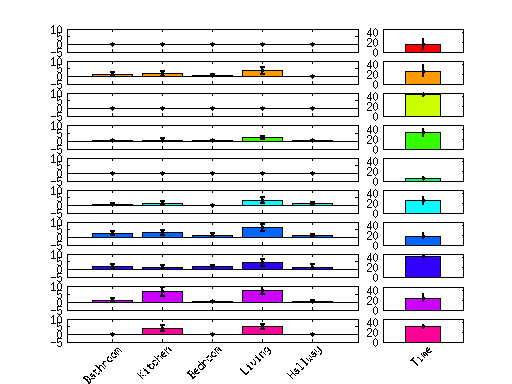
\includegraphics[width=\textwidth]{Pictures/Gaus/TopHN1TS48k20.png}
 \end{minipage}
 \caption{Topic distribution per day and the Topic visualization for LDA-Gaussian. HouseNr=1}
\end{figure}

\begin{figure}
 \centering
 \begin{minipage}[b]{0.45\linewidth}
  \centering
  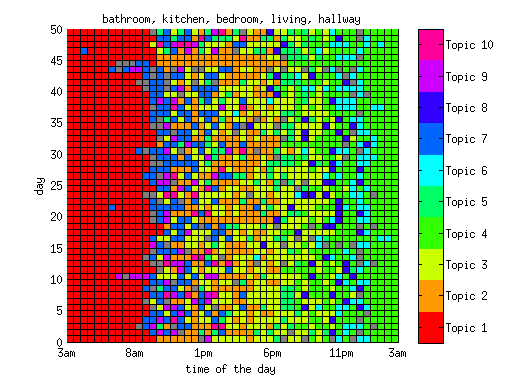
\includegraphics[width=\textwidth]{Pictures/Pois/DayHN1TS48k20.png}
 \end{minipage}
 \begin{minipage}[b]{0.45\linewidth}
  \centering
  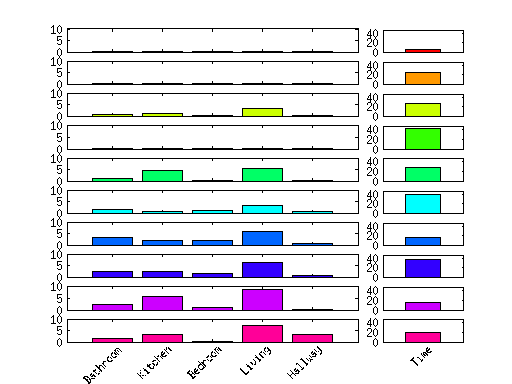
\includegraphics[width=\textwidth]{Pictures/Pois/TopHN1TS48k20.png}
 \end{minipage}
 \caption{Topic distribution per day and the Topic visualization for LDA-Poisson. HouseNr=1}
\end{figure}
%----------------------------------------------------------------------------
%HN=2
\begin{figure}
 \centering
 \begin{minipage}[b]{0.45\linewidth}
  \centering
  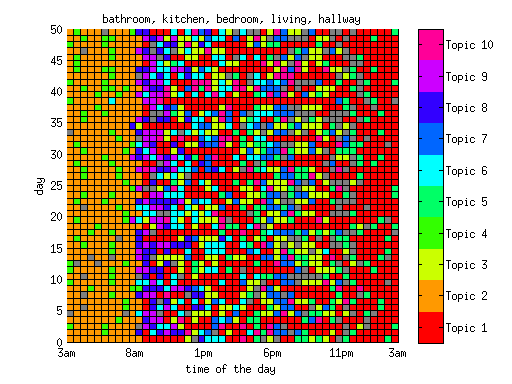
\includegraphics[width=\textwidth]{Pictures/Gaus/DayHN2TS48k20.png}
 \end{minipage}
 \begin{minipage}[b]{0.45\linewidth}
  \centering
  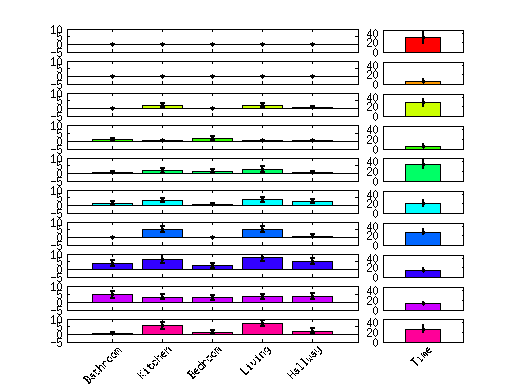
\includegraphics[width=\textwidth]{Pictures/Gaus/TopHN2TS48k20.png}
 \end{minipage}
 \caption{Topic distribution per day and the Topic visualization for LDA-Gaussian. HouseNr=2}
\end{figure}

\begin{figure}
 \centering
 \begin{minipage}[b]{0.45\linewidth}
  \centering
  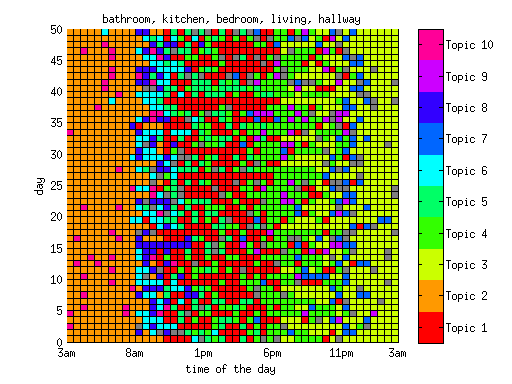
\includegraphics[width=\textwidth]{Pictures/Pois/DayHN2TS48k20.png}
 \end{minipage}
 \begin{minipage}[b]{0.45\linewidth}
  \centering
  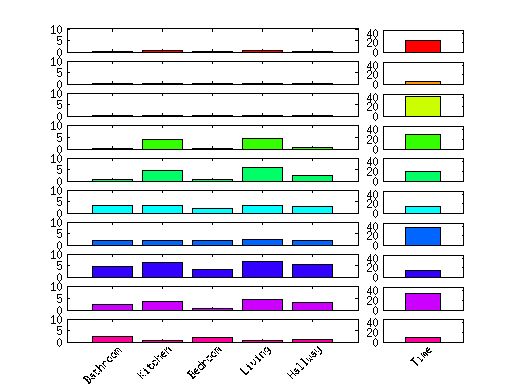
\includegraphics[width=\textwidth]{Pictures/Pois/TopHN2TS48k20.png}
 \end{minipage}
 \caption{Topic distribution per day and the Topic visualization for LDA-Poisson. HouseNr=2}
\end{figure}

%---------------------------------------------------------
%HN=3

\begin{figure}
 \centering
 \begin{minipage}[b]{0.45\linewidth}
  \centering
  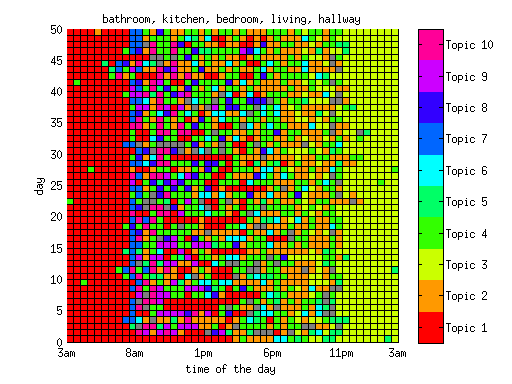
\includegraphics[width=\textwidth]{Pictures/Gaus/DayHN3TS48k20.png}
 \end{minipage}
 \begin{minipage}[b]{0.45\linewidth}
  \centering
  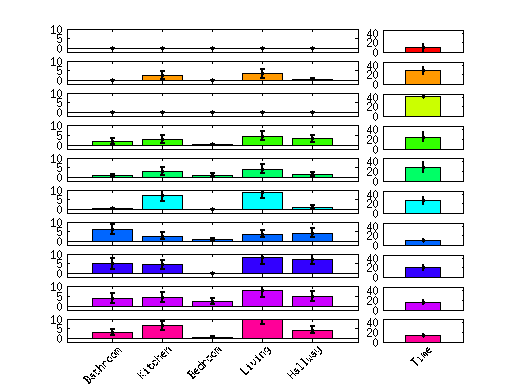
\includegraphics[width=\textwidth]{Pictures/Gaus/TopHN3TS48k20.png}
 \end{minipage}
 \caption{Topic distribution per day and the Topic visualization for LDA-Gaussian. HouseNr=3}
\end{figure}

\begin{figure}
 \centering
 \begin{minipage}[b]{0.45\linewidth}
  \centering
  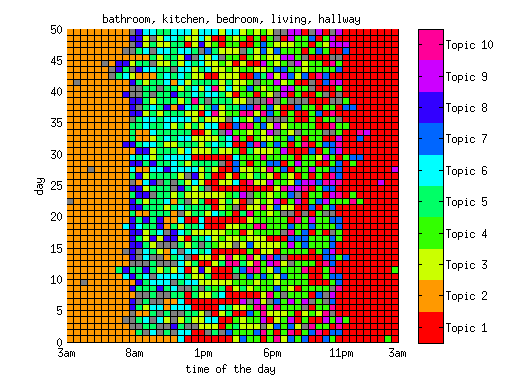
\includegraphics[width=\textwidth]{Pictures/Pois/DayHN3TS48k20.png}
 \end{minipage}
 \begin{minipage}[b]{0.45\linewidth}
  \centering
  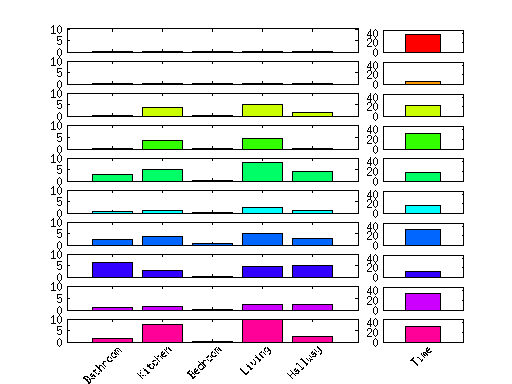
\includegraphics[width=\textwidth]{Pictures/Pois/TopHN3TS48k20.png}
 \end{minipage}
 \caption{Topic distribution per day and the Topic visualization for LDA-Poisson. HouseNr=3}
\end{figure}
%----------------------------------------------------------------------------
%HN=4

\begin{figure}
 \centering
 \begin{minipage}[b]{0.45\linewidth}
  \centering
  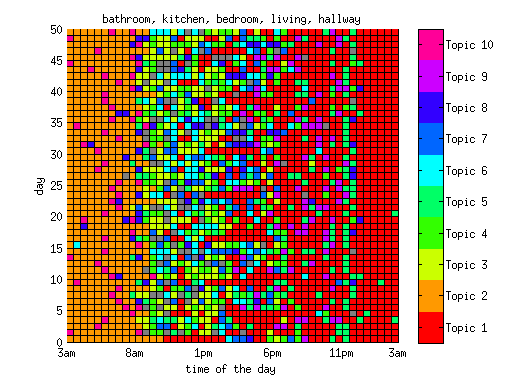
\includegraphics[width=\textwidth]{Pictures/Gaus/DayHN4TS48k20.png}
 \end{minipage}
 \begin{minipage}[b]{0.45\linewidth}
  \centering
  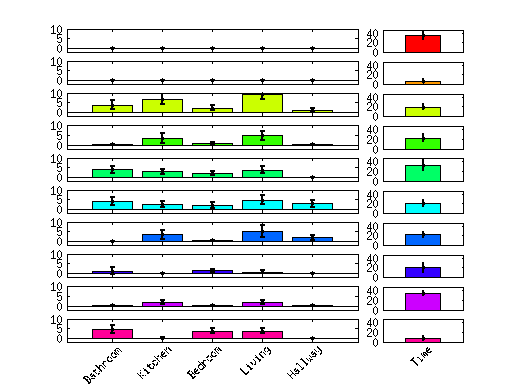
\includegraphics[width=\textwidth]{Pictures/Gaus/TopHN4TS48k20.png}
 \end{minipage}
 \caption{Topic distribution per day and the Topic visualization for LDA-Gaussian. HouseNr=4}
\end{figure}

\begin{figure}
 \centering
 \begin{minipage}[b]{0.45\linewidth}
  \centering
  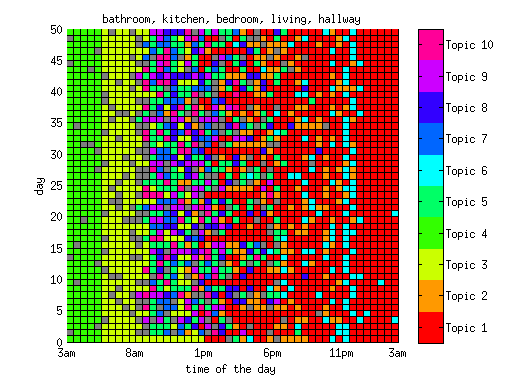
\includegraphics[width=\textwidth]{Pictures/Pois/DayHN4TS48k20.png}
 \end{minipage}
 \begin{minipage}[b]{0.45\linewidth}
  \centering
  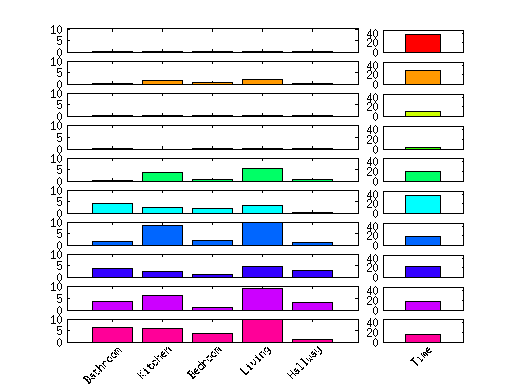
\includegraphics[width=\textwidth]{Pictures/Pois/TopHN4TS48k20.png}
 \end{minipage}
 \caption{Topic distribution per day and the Topic visualization for LDA-Poisson. HouseNr=4}
\end{figure}
%-----------------------------------------------------------------------------
%HN=5

\begin{figure}
 \centering
 \begin{minipage}[b]{0.45\linewidth}
  \centering
  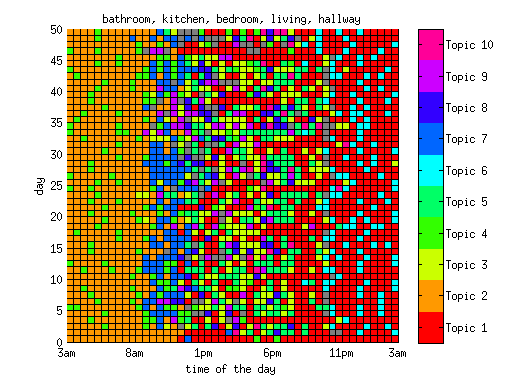
\includegraphics[width=\textwidth]{Pictures/Gaus/DayHN5TS48k20.png}
 \end{minipage}
 \begin{minipage}[b]{0.45\linewidth}
  \centering
  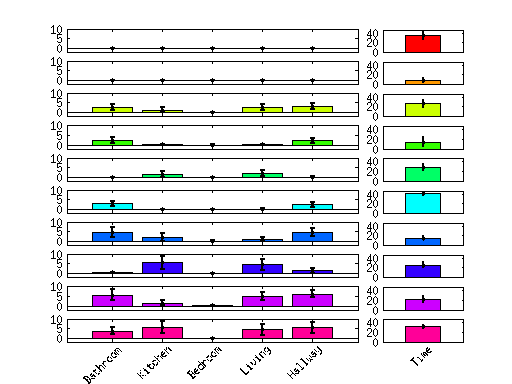
\includegraphics[width=\textwidth]{Pictures/Gaus/TopHN5TS48k20.png}
 \end{minipage}
 \caption{Topic distribution per day and the Topic visualization for LDA-Gaussian. HouseNr=5}
\end{figure}

\begin{figure}
 \centering
 \begin{minipage}[b]{0.45\linewidth}
  \centering
  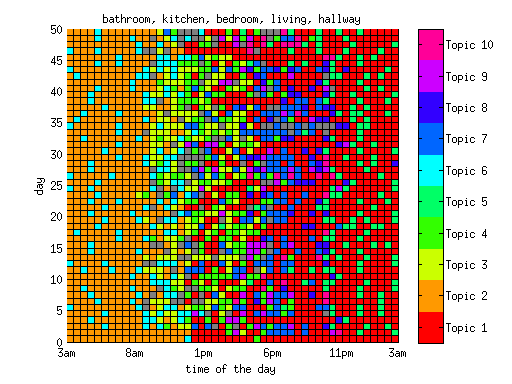
\includegraphics[width=\textwidth]{Pictures/Pois/DayHN5TS48k20.png}
 \end{minipage}
 \begin{minipage}[b]{0.45\linewidth}
  \centering
  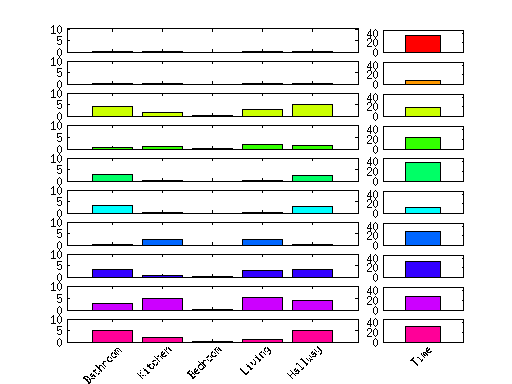
\includegraphics[width=\textwidth]{Pictures/Pois/TopHN5TS48k20.png}
 \end{minipage}
 \caption{Topic distribution per day and the Topic visualization for LDA-Poisson. HouseNr=5}
\end{figure}

You can see that for some people the structure of their daily behavior is more easily found than for other people. And also the different model give slightly different results.
For some people you can clearly see the topic 'Going to toilet at night`. For house number 4 this topic is marked with pink in the LDA-Gaussian model. The three fields bathroom, bedroom and living are active and the mean time value is quiet low, which corresponds with an early time. For house number one this topic is also captured in the LDA Gaussian model, but not in the LDA-Poisson model.\\
You can also see the different behavior patterns between the persons. For example the person of house number 5 tends to sleep a little bit longer than the persons of other houses. Some behaviors are more regular than others.
The LDA-Poisson model tends to focus on the time a little bit more then the LDA-Gaussian model.


\pagebreak

\subsection{Quantitative Results}
To see if our results not only hold on our training data we we wish to also find a high log-likelihood for a hold-out set. In this way we make sure that the model does not over-fit the data. So for a given hold-out set we can calculate the perplexity with 

\begin{equation}
 perplexity(D_{HOS}) = exp \left\{ - \frac{\sum_{m=1}^M \log p(\textbf{o}_d ) }{M*N} \right\}
\end{equation}

In the next experiments we use 10\% percent of our data as a hold-out set. We train the model on the rest of the data for different initialization values and calculate the perplexity for every run.

\paragraph{Different Sets of Data}
In figure \ref{fig:PerplGaus} the perplexity is shown for the 5 different data-sets gained from the 5 houses. Every run is performed ten times and we took the mean over these runs for every initialization of amount of topics $k$. Every run is initialized with 5 days.
The data sets vary in length, but as you can see in the figure, the amount of data is not necessary of influence how well the LDA-Gaussian model can be trained. Some data sets are much more stable than others and this is probably due to the way how regular peoples behavior is.

\begin{figure}[h!]
 \centering
 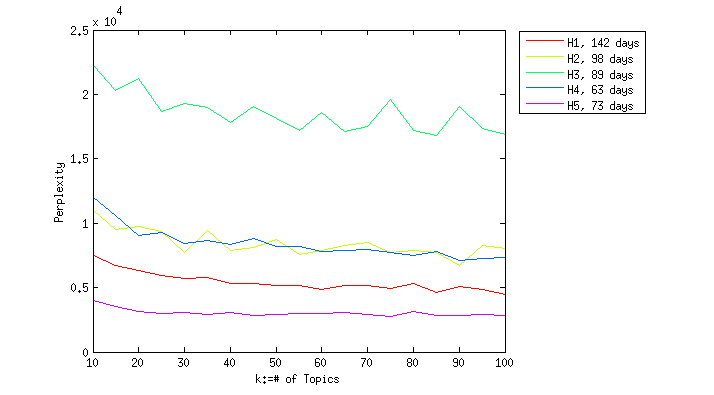
\includegraphics[width=0.7\textwidth]{Pictures/PerplGaus.png}
 \caption{Perplexity for different initializations of Topics for 5 different House}
 \label{fig:PerplGaus}
\end{figure}

\paragraph{Comparison LDA-Gaussian and LDA-Poisson}

To compare the two models with each other we drop the time dimensions in the observations and calculate the perplexity for the hold-out set with different amount of time-slices (figure \ref{fig:CompareTS}) and with different amount of topics (figure \ref{fig:CompareK}).
You can see that the LDA-Gaussian model outperforms the LDA-Poisson model for small amount of time-slices as well as for small amount of topics. When the amount of time-slices increases the performance of both models becomes similar to each other. 

\begin{figure}[h!]
 \centering
 \begin{minipage}[b]{0.45\linewidth}
  \centering
  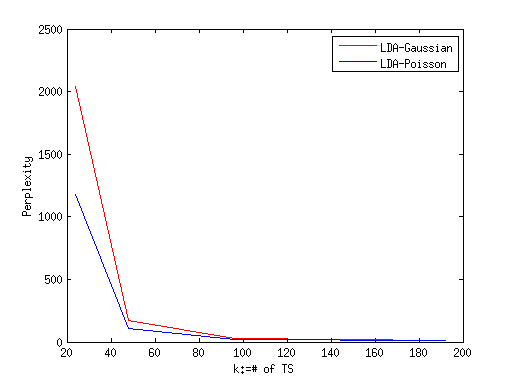
\includegraphics[width=\textwidth]{Pictures/CompareTSgausPois.png}
  \caption{Perplexity for LDA-Gaussian and LDA-Poisson with different amount of time-slices}
  \label{fig:CompareTS}
 \end{minipage}
 \begin{minipage}[b]{0.45\linewidth}
  \centering
  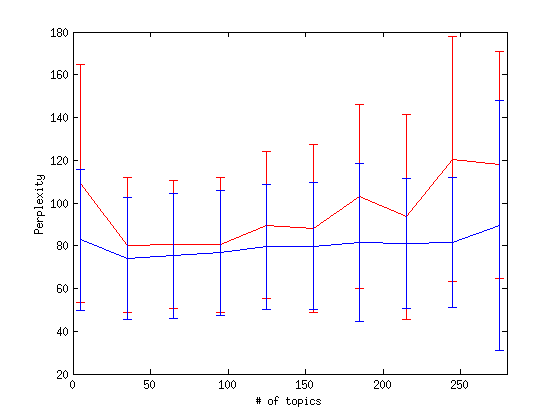
\includegraphics[width=\textwidth]{Pictures/CompareCrossTops.png}
\caption{Perplexity for LDA-Gaussian and LDA-Poisson with different amount of topics}
  \label{fig:CompareK}
 \end{minipage}
 \caption{}
 \label{fig:Compare}
\end{figure}


\paragraph{Different length of time-slices}

In figure \ref{fig:PerplTS} we give the perplexity for different length of time-slices for the 5 Houses. We take a again the mean over 10 runs. We take for every house the same amount of days to train and test the data. We can see that with more time-slices the perplexity becomes lower for the hold-out set. For house $H2$ and $H4$ the perplexity is much better for a small amount of time-slices. The perplexities for these two houses drop much faster if the amount of time-slices increases.

\begin{figure}[h!]
 \centering
 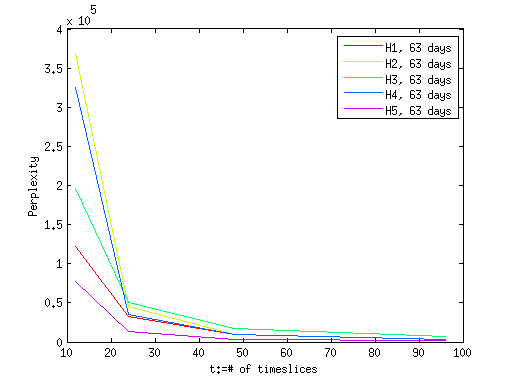
\includegraphics[width = 0.7\textwidth]{Pictures/PerplTS.png}
 \caption{Perplexity (x-axis) for the hold-out-set for different amount of time-slices (y-axis)}
 \label{fig:PerplTS}
\end{figure}